\documentclass[adraft,creativecommons]{eptcs}
\usepackage[utf8]{inputenc}

\usepackage{underscore}

\usepackage[T1]{fontenc}
\usepackage{mathpartir}
\usepackage{amssymb}
\usepackage{amsmath}
\usepackage{braket}
\usepackage{xspace}
\usepackage[capitalize]{cleveref}
\crefformat{section}{\S#2#1#3}
% \crefformat{figure}{Fig. #2#1#3}

% \usepackage{adjustbox}
\usepackage{tikz}
\usetikzlibrary{quantikz}

% From: https://tomhennigan.blogspot.com/2012/01/grouped-emails-in-latex-with-href-and.html
\newcommand{\mailtodomain}[1]{\href{mailto:#1}{\nolinkurl{#1}}}

\usepackage{xcolor}
\definecolor{dkgreen}{rgb}{0,0.35,0}

\usepackage{listings}
\lstloadlanguages{Haskell}
\lstdefinelanguage{QHaskell}{
    language     = Haskell,
    morekeywords = {bool, qbit, U, C, meas, apply, to},
}

\lstset{
    basicstyle=\small\ttfamily,
    frame=single,
    captionpos=b,
    numbers=left,
    numberstyle=\tiny\color{gray},
    flexiblecolumns=false,
    basewidth={0.5em,0.5em},
    commentstyle=\color{dkgreen},
    keywordstyle=\bfseries\color{blue},
    stringstyle=\color{violet},
    literate=
        {√}{{$\surd$}}1
        {>}{{$>$}}1 {<}{{$<$}}1
        {\\\\}{{\char`\\\char`\\}}1
        {⇐}{{$\Leftarrow$}}1 {⇒}{{$\Rightarrow$}}2
        {->}{{$\rightarrow$}}2
        {\ .}{{$\circ$}}2 {\ .\ }{{$\circ$}}2
        {|}{{$\vert$}}1 {⟩}{{$\rangle$}}1
        {∧}{{$\wedge$}}1 {∨}{{$\vee$}}1
        {∈}{{$\in$}}1 {Π}{{$\Pi$}}1 {∃}{{$\exists$}}1
        {⊗}{{$\otimes$}}1 {⊕}{{$\oplus$}}1
        {⊤}{{$\top$}}2
        {=q}{{$=_q$}}2 {=c}{{$=_c$}}2
        {α}{{$\alpha$}}1 {β}{{$\beta$}}1
        {_i}{{$_i$}}1
        {\ .\ }{{$\cdot$}}1
        {β00}{{$\beta_{00}$}}2
}

\usepackage{blindtext}

\def\titlerunning{Quantum Hoare Type Theory}
\def\authorrunning{Kartik Singhal}

\title{\titlerunning}

\author{
Kartik Singhal
\institute{University of Chicago}
\email{\mailtodomain{ks@cs.uchicago.edu}}
}

\begin{document}

\maketitle

\thispagestyle{empty}

\tableofcontents

\listoffigures

\lstlistoflistings

\listoftables

\clearpage

\pagenumbering{arabic}

\section{Introduction}

\blindtext

\section{Background}

TODO:

- Hoare logic and Hoare Type Theory

- basics of quantum computing

- Quantum Hoare Logic

- define the meaning of subspace/projector-based predicates/propositions.

\section{Quantum Hoare Type Theory}

TODO:

- define the syntax of the language

- proof rules at each step

\subsection{Examples}

\blindtext

\subsubsection{Bell states}

Our simplest example involves creation of a Bell (or EPR) state which is one of the four maximally entangled quantum states of two qubits. Specifically, we will create a circuit (\cref{fig:bell00}) to produce the first Bell state which we will write in the mnemonic notation as $\ket{\beta_{00}} = (\ket{00}+\ket{11})/\sqrt{2}$.

\begin{figure}[b]
    \centering
    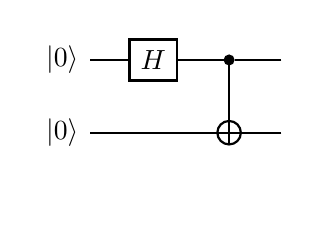
\begin{tikzpicture}
        \node[scale=1.0] {
            \begin{quantikz}
                \lstick{$\ket{0}$} & \gate{H} & \ctrl{1} & \qw \\
                \lstick{$\ket{0}$} & \qw      & \targ{}  & \qw \\
            \end{quantikz}
        };
    \end{tikzpicture}
    \caption{Circuit to produce the first Bell state}
    \label{fig:bell00}
\end{figure}

\lstinputlisting[language=QHaskell,lastline=7,caption=Generating Bell state]{bell00.qh}

This corresponds to a suspended quantum computation (or a quantum circuit) that can be composed with other computations (circuits). The specification of the program is in its type (the first line). Here we see our first two propositions: the top, $\top$, predicate that is satisfied by any state space and the $X =_q \ket{\psi}$ predicate that is satisfied by quantum variables, $X$, that lie in the span of the given state $\ket{\psi}$. Intuitively, this circuit does not require any inputs and can work in any given state space and produces two qubits that are maximally entangled in the first Bell state $\ket{\beta_{00}}$.

Here is how we can prove whether this program conforms to the given specification.

\lstinputlisting[language=QHaskell,firstline=9,caption=Bell state program annotated with propositions]{bell00.qh}

\section{Discussion and Related Work}

\blindtext

\section{Conclusion and Perspectives}

\blindtext

\bibliographystyle{eptcsalpha}

\end{document}
